\documentclass{article}
\usepackage{amsmath}
\usepackage{listings}
\usepackage{xcolor}
\usepackage{graphicx}
\usepackage[margin=0.75in]{geometry}



\title{Understanding AI Agents and Their Interaction with Complex Environments}
\author{Muhammad Abdullah (22P-9371)}
\date{February 2025}

\begin{document}

\maketitle

\textbf{\large Scenario: AI in Autonomous Maritime Navigation}\\
Maritime shipping is critical for global trade, yet it faces challenges like unpredictable weather, congested shipping lanes, and collision risks. Companies are developing AI-powered autonomous ships to navigate the oceans with minimal human intervention.

\section{Agent Perspective}
\subsection{AI Agent Classification and Implementation}
The best AI agent for an autonomous ship is a combination of Model-Based Reflex, Goal-Based, and Utility-Based Agents.

\subsubsection{Model-Based Reflex Agent}
\textbf{Reasoning:} The ship must respond to immediate changes in its environment while maintaining an internal model of the world. The Model-Based Reflex Agent is ideal because it can track the current state and update its model using real-time data.

\textbf{Perception Mechanisms:}
\begin{itemize}
    \item \textbf{Radar:} Detects nearby ships and obstacles, particularly in low visibility conditions like fog.
    \item \textbf{Cameras:} Provides visual data for detecting other ships, navigation buoys, or hazards.
    \item \textbf{LIDAR:} Maps the surrounding environment in 3D, detecting obstacles and other vessels.
    \item \textbf{Sonar:} Detects underwater obstacles, ensuring safe navigation near shallow areas or in ports.
    \item \textbf{GPS and IMU:} Tracks the ship's position, speed, and orientation to ensure it follows the correct path.
\end{itemize}

\subsubsection{Goal-Based Agent}
\textbf{Reasoning:} The ship must achieve the goal of safely reaching its destination. The Goal-Based Agent is responsible for planning and adjusting actions to ensure the primary goal is met.

\textbf{Perception Mechanisms:} Uses the same sensor data (radar, cameras, LIDAR, etc.) to monitor conditions that may impact the goal, such as nearby traffic or adverse weather, and adjusts the route accordingly.

\subsubsection{Utility-Based Agent}
\textbf{Reasoning:} The ship needs to evaluate trade-offs between different objectives (e.g., safety vs. time). The Utility-Based Agent helps in decision-making when there are competing goals, such as optimizing fuel consumption, travel time, and avoiding risks.

\textbf{Perception Mechanisms:} Similar sensors (radar, cameras, LIDAR, etc.) are used to assess risks and calculate the best route, considering the balance of utility factors like fuel efficiency and safety.

\subsubsection{Justification}
The Model-Based Reflex Agent allows the ship to react to its environment using real-time data from sensors. The Goal-Based Agent enables the ship to achieve its mission, and the Utility-Based Agent allows for optimal decision-making when there are multiple objectives. Combining these agents gives the ship the ability to both respond to immediate changes and plan long-term actions while balancing trade-offs effectively.

\subsubsection{Code Implementation}
\begin{lstlisting}[language=Python, caption={AI Agent for Autonomous Ship Navigation}]
import random

class Percept:
    # Represents the data received from sensors.
    def __init__(self, obstacle_distance, weather_condition, traffic_density, fuel_level):
        self.obstacle_distance = obstacle_distance  
        self.weather_condition = weather_condition 
        self.traffic_density = traffic_density 
        self.fuel_level = fuel_level

class ShipAgent:
    # AI agent that makes navigation decisions based on percepts.
    def __init__(self, destination="Port B"):
        self.speed = 20  
        self.direction = 'Straight'
        self.internal_state = {}  # Stores past observations
        self.destination = destination  # Goal-Based Behavior
    
    def update_model(self, percept):
        # Updates internal world model with new percept data.
        self.internal_state['last_weather'] = percept.weather_condition
        self.internal_state['last_obstacle_distance'] = percept.obstacle_distance
    
    def calculate_utility(self, percept):
        # Evaluates different options to maximize efficiency and safety.
        utility = 100  # Start with max utility
        
        # Safety factor
        if percept.obstacle_distance < 50:
            utility -= 50  # High penalty for close obstacles
        
        # Efficiency factor (fuel level)
        if percept.fuel_level < 20:
            utility -= 30  # Penalize low fuel levels
        
        # Time factor (traffic congestion)
        if percept.traffic_density > 7:
            utility -= 20  # Slow navigation reduces efficiency
        
        return utility

    def agent_program(self, percept):
        # Decision-making based on percepts, goals, and utility.
        self.update_model(percept)  # Update internal state

        # Adjust speed based on weather conditions
        if percept.weather_condition == 'Stormy':
            self.speed = max(5, self.speed - 10)  
        elif percept.weather_condition == 'Foggy':
            self.speed = max(10, self.speed - 5)
        else:
            self.speed = min(25, self.speed + 5) 
        
        # Avoid collision if an obstacle is too close
        if percept.obstacle_distance < 50:
            self.direction = 'Turn Left'
        elif percept.obstacle_distance < 100:
            self.direction = 'Turn Right'
        else:
            self.direction = 'Straight'
        
        # Adjust speed based on traffic density
        if percept.traffic_density > 5:
            self.speed = max(10, self.speed - 5)

        # Use utility-based decision-making
        utility = self.calculate_utility(percept)
        if utility < 50:
            self.speed = max(5, self.speed - 5)  # Slow down for safety
        
        return f"Speed: {self.speed} knots, Direction: {self.direction}, 
        Utility Score: {utility}, Destination: {self.destination}"

for _ in range(5): 
    obstacle_distance = random.randint(10, 500)  
    weather_condition = random.choice(['Clear', 'Foggy', 'Stormy'])
    traffic_density = random.randint(0, 10)  
    fuel_level = random.randint(10, 100)  # New: Fuel level added
    
    percept = Percept(obstacle_distance, weather_condition, traffic_density, fuel_level)
    ship = ShipAgent()
    decision = ship.agent_program(percept)
    
    print(f"Percepts -> Obstacle: {percept.obstacle_distance}m, 
    Weather: {percept.weather_condition}, Traffic: {percept.traffic_density}, 
    Fuel: {percept.fuel_level}%")
    print(f"Decision -> {decision}\n")
\end{lstlisting}
\subsubsection{Output}
Here is the screenshot of the program's output:

\begin{figure}[h!]
    \centering
    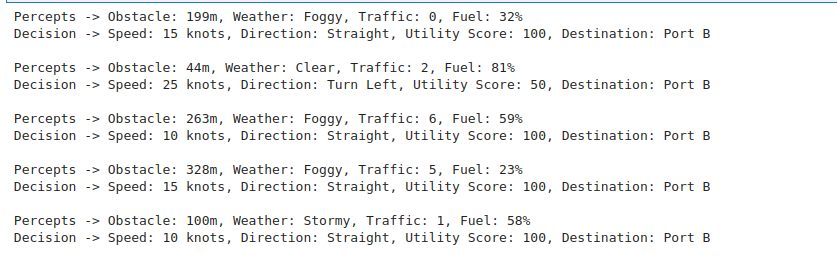
\includegraphics[width=0.7\textwidth]{1_a.png} 
    \caption{Screenshot of the output}
\end{figure}

\subsection{Data Integration in the AI System}
The autonomous ship’s AI continuously gathers and processes environmental data from various sources to ensure safe and efficient navigation. These sources provide information about positioning, obstacles, weather conditions, and traffic awareness.

\textbf{GPS (Satellite Positioning)}
\begin{itemize}
    \item Determines the ship’s exact location using latitude and longitude.
    \item Compares the current position with the planned route to ensure the ship follows the most efficient path.
    \item Priority Level: Low (Used for long-term navigation, not for immediate threat response).
\end{itemize}

\textbf{Radar (Above-Water Obstacle Detection)}
\begin{itemize}
    \item Detects ships, buoys, landmasses, and floating debris to prevent collisions.
    \item Provides real-time data on nearby objects, enabling quick decision-making.
    \item Priority Level: High (Immediate obstacle avoidance is the highest priority).
\end{itemize}

\textbf{Sonar (Underwater Obstacle Detection)}
\begin{itemize}
    \item Identifies underwater hazards such as icebergs, reefs, and marine life.
    \item Works in conjunction with radar to avoid submerged threats.
    \item Priority Level: High (Prevents collisions with underwater objects).
\end{itemize}

\textbf{Weather Forecast Data (Weather Adaptation)}
\begin{itemize}
    \item Provides real-time updates on storm conditions, fog, heavy winds, and waves.
    \item Helps adjust the ship’s speed to avoid dangerous conditions.
    \item Priority Level: Medium (Affects speed rather than direction).
\end{itemize}

\textbf{AIS (Automatic Identification System - Traffic Awareness)}
\begin{itemize}
    \item Tracks other ships’ positions, speeds, and routes to avoid congestion.
    \item Helps in route adjustments to prevent collisions in busy shipping lanes.
    \item Priority Level: Medium (Ensures compliance with maritime traffic rules).
\end{itemize}

\subsubsection{How the AI Prioritizes and Filters Data}
The AI system processes incoming data in a hierarchical manner, ensuring that the most urgent safety concerns are addressed first.

\textbf{First Priority: Immediate Collision Avoidance (Radar and Sonar)}
\begin{itemize}
    \item If above-water or underwater obstacles are detected within a critical range, the AI immediately adjusts the ship’s direction to avoid a collision.
    \item Speed is significantly reduced if the obstacle is very close.
    \item This takes absolute priority over all other considerations.
\end{itemize}

\textbf{Second Priority: Weather Adaptation (Weather Forecast)}
\begin{itemize}
    \item If weather conditions are stormy or foggy, the AI reduces speed to improve stability and visibility.
    \item The direction remains unchanged unless required by obstacle avoidance.
\end{itemize}

\textbf{Third Priority: Traffic Avoidance (AIS - Nearby Ships)}
\begin{itemize}
    \item If another vessel is detected within a critical range, the AI adjusts course to maintain a safe distance.
    \item Speed is gradually reduced to prevent collisions.
    \item This ensures compliance with maritime traffic rules.
\end{itemize}

\textbf{Fourth Priority: Route Optimization (GPS Guidance)}
\begin{itemize}
    \item When no immediate obstacles exist, the AI optimizes the speed and direction based on the planned GPS route.
    \item Speed is increased up to a safe limit to maintain efficiency.
\end{itemize}

\subsubsection{\large High-Level Decision-Making Model}
The AI follows a structured decision-making model based on these priorities:

\begin{enumerate}
    \item Is there an immediate risk of collision?
    \begin{itemize}
        \item Yes: Adjust direction immediately. Reduce speed significantly.
        \item No: Proceed to the next step.
    \end{itemize}
    \item Are weather conditions affecting safety?
    \item Is there traffic congestion nearby?
    \item Can we optimize the route for efficiency?
\end{enumerate}
\subsubsection{Code Implementation}
\begin{lstlisting}[language=Python, caption={AI Agent for Autonomous Ship Navigation}]
import random

class ShipAI:
    #AI system that integrates multiple data sources for navigation decisions.
    def __init__(self):
        self.speed = 20  
        self.direction = 'Straight'
    
    def process_data(self, gps, radar, sonar, weather, ais):
        """
        Prioritizes and filters data to ensure safe navigation.
        - High Priority: Immediate obstacle avoidance (Radar, Sonar).
        - Medium Priority: Weather adaptation (Weather forecast).
        - Medium Priority: Traffic avoidance (AIS - Automatic Identification System).
        - Low Priority: Route optimization (GPS guidance).
        """
        
        # 1. High-Priority: Immediate Collision Avoidance (Radar & Sonar)
        if radar < 50 or sonar < 30:
            self.direction = 'Turn Left' if radar < sonar else 'Turn Right'
            self.speed = max(5, self.speed - 10)  
        
        # 2. Medium-Priority: Weather Adaptation
        elif weather in ['Stormy', 'Foggy']:
            self.speed = max(10, self.speed - 5)  
        
        # 3. Medium-Priority: Traffic Avoidance (AIS - Nearby Ships)
        elif ais < 100:  # If another ship is within 100m
            self.direction = 'Adjust Course'
            self.speed = max(10, self.speed - 5)  
        
        # 4. Low-Priority: Route Optimization (GPS Guidance)
        else:
            self.direction = 'Straight'
            self.speed = min(25, self.speed + 5)  
        
        return f"Speed: {self.speed} knots, Direction: {self.direction}"


test_cases = [
    ((37.7749, -122.4194), 120, 200, 'Clear', 150),  # No obstacles, normal weather
    ((40.7128, -74.0060), 30, 50, 'Foggy', 80),  # Close obstacle + bad weather + traffic
    ((34.0522, -118.2437), 70, 20, 'Stormy', 200),  # Underwater obstacle + storm
    ((51.5074, -0.1278), 45, 100, 'Clear', 90),  # Close radar obstacle, adjust course
    ((48.8566, 2.3522), 150, 250, 'Clear', 300)  # Safe conditions, optimize speed
]

# Simulating AI decisions
ship_ai = ShipAI()
for i, case in enumerate(test_cases, 1):
    decision = ship_ai.process_data(*case)
    print(f"Test Case {i}: Navigation Decision -> {decision}")

\end{lstlisting}
\subsubsection{Output}
Here is the screenshot of the program's output:

\begin{figure}[h!]
    \centering
    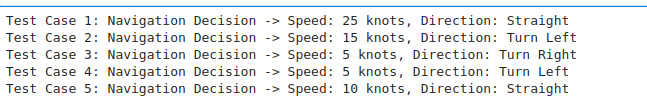
\includegraphics[width=0.7\textwidth]{1_b.png} 
    \caption{Screenshot of the output}
\end{figure}
\subsection{Single vs. Multi-Agent Systems for Autonomous Ships}

\subsubsection{\large Should an Autonomous Ship Operate as a Single or Multi-Agent System?}

An autonomous ship can function as either a single intelligent agent or as part of a multi-agent system (MAS), depending on the operational complexity and communication requirements.

\subsubsection{Single-Agent System (Standalone AI)}
In a single-agent system, each ship makes independent decisions using its own onboard AI, sensors, and data sources. The ship does not communicate with other ships or port authorities in real time but instead relies on pre-existing navigational rules and its perception of the environment.

\paragraph{Pros of a Single-Agent System:}
\begin{itemize}
    \item Simpler implementation (No need for communication protocols).
    \item More resilient to network failures or external system downtime.
    \item Reduces dependency on external data, making it self-sufficient.
\end{itemize}

\paragraph{Cons of a Single-Agent System:}
\begin{itemize}
    \item Cannot coordinate with other ships, increasing collision risks in congested areas.
    \item Lacks shared situational awareness, which is critical in complex maritime environments.
\end{itemize}

\subsubsection{Multi-Agent System (MAS) with Communication}
A multi-agent system consists of autonomous ships, port authorities, and traffic control systems, all communicating and coordinating their actions in real time. This system enables ships to exchange position, speed, weather conditions, and congestion data, improving navigation efficiency and safety.

\paragraph{Pros of a Multi-Agent System:}
\begin{itemize}
    \item Better collision avoidance – Ships exchange location data to prevent accidents.
    \item Traffic coordination – Ships adjust their routes to avoid congested areas.
    \item Improved route optimization – Ships receive live updates on weather conditions and traffic.
    \item Regulatory compliance – Ships can communicate with maritime authorities for real-time adjustments.
\end{itemize}

\paragraph{Cons of a Multi-Agent System:}
\begin{itemize}
    \item Requires network infrastructure (satellite, VHF, or 5G communication).
    \item Increased cybersecurity risks from data sharing.
    \item More complex implementation and dependency on reliable communication channels.
\end{itemize}

\subsubsection{\large Real-World Maritime Challenges That Influence This Decision}
\begin{itemize}
    \item \textbf{Congested Shipping Lanes} – Many vessels in busy areas (e.g., the Panama Canal) require coordinated navigation to avoid collisions.
    \item \textbf{Varying Weather Conditions} – Ships need real-time weather updates from each other to optimize speed and routes.
    \item \textbf{Emergency Handling} – In case of distress, coordinated assistance is required from nearby vessels and authorities.
    \item \textbf{Port Entry \& Docking} – Multi-agent communication with port authorities helps optimize docking schedules and avoid congestion.
    \item \textbf{Cybersecurity Risks} – A connected system introduces hacking threats, requiring secure communication protocols.
\end{itemize}

\subsubsection{Conclusion}
A multi-agent system is the preferred choice in complex environments where coordination is necessary, but standalone AI works for less crowded, open-sea navigation.

\subsubsection{\large Multi-Agent System Architecture for Ship Communication}

A multi-agent architecture consists of:
\begin{itemize}
    \item \textbf{Ship Agents} – Autonomous ships that communicate their positions and receive navigation updates.
    \item \textbf{Port Authority Agents} – Monitors traffic, weather, and docking schedules.
    \item \textbf{Traffic Control Center} – Ensures compliance with maritime traffic rules.
\end{itemize}

Each agent communicates using a secure API-based system over satellite or 5G networks.

\paragraph{Key Features of This Implementation:}
\begin{itemize}
    \item Uses HTTP-based API communication for easy integration.
\end{itemize}

\subsubsection{Sample Code Snippet}

Here’s how two ships can communicate with each other to exchange positions:

\subsubsection{Ship 2: (Receiver)}

\begin{verbatim}
from flask import Flask, request, jsonify

app = Flask(__name__)

@app.route('/receive_position', methods=['POST'])
def receive_position():  # Agent function
    # Receive and process ship position data.
    data = request.json
    ship_id = data.get("ship_id")
    position = data.get("position")
    print(f"Received Position from {ship_id}: {position}")
    return jsonify({"status": "Position received"}), 200

if __name__ == '__main__':
    app.run(port=5000)
\end{verbatim}

\subsubsection{Ship 1: (Sender)}

\begin{verbatim}
import requests

class ShipAgent:
    def __init__(self, ship_id, position):
        self.ship_id = ship_id
        self.position = position  # (latitude, longitude)

    def send_position(self, target_url):  # Agent function
        # Send ship position to another ship or port authority.
        data = {'ship_id': self.ship_id, 'position': self.position}
        response = requests.post(target_url, json=data)
        print(f"Sent Position: {self.position} | Response: {response.text}")

ship1 = ShipAgent("Ship_1", (37.7749, -122.4194))
ship2 = ShipAgent("Ship_2", (55.76789, -102.98789))
target_url = "http://127.0.0.1:5000/receive_position"  # Ship 2's server
ship1.send_position(target_url)
ship2.send_position(target_url)
\end{verbatim}

This basic setup allows one ship to send its position to another. This can be extended to include additional data, such as weather conditions, speed, and route updates, further enhancing the capabilities of a multi-agent system.

\subsubsection{Final Thoughts}
For simple navigation, a single-agent system may be sufficient. However, for safer, smarter maritime transport, a multi-agent system is essential. It enables ship-to-ship and ship-to-port communication, which can lead to improved coordination and efficiency in complex maritime environments.
Here is the screenshot of the program's output:

\begin{figure}[h!]
    \centering
    
\includegraphics[width=0.7\textwidth]{1_c.png} 
    \caption{Screenshot of the output}
\end{figure}
\section{Classifying the Oceanic Environment}

\subsection{Classifying the Oceanic Environment in Terms of Observability, Determinism, and Dynamism}

\subsubsection{Observability}
\textbf{Definition:} Observability refers to the extent to which the agent (in this case, the ship) can access information about its environment.

\textbf{Oceanic Environment Observability:} The oceanic environment is partially observable. While certain aspects like weather conditions, visibility, and obstacle density can be observed via sensors and cameras, the ship cannot always fully perceive underwater objects, distant hazards, or sudden changes in conditions.

\textbf{Challenges for AI:} Since the environment is not fully observable, the AI system may need to make decisions based on incomplete information, requiring sophisticated prediction models and the ability to handle uncertainty in the data.

\subsubsection{Determinism}
\textbf{Definition:} Determinism refers to whether the future states of the environment are completely determined by the current state and the actions taken.

\textbf{Oceanic Environment Determinism:} The oceanic environment is non-deterministic. Factors like weather patterns, ocean currents, and unexpected obstacles (e.g., submerged rocks or sudden storms) make it impossible to predict the exact future state based on the current state alone.

\textbf{Challenges for AI:} Non-determinism introduces unpredictability, meaning the AI must be equipped with reactive decision-making capabilities to handle sudden changes in the environment and adapt its behavior dynamically.

\subsubsection{Dynamism}
\textbf{Definition:} Dynamism refers to how quickly the environment changes over time.

\textbf{Oceanic Environment Dynamism:} The oceanic environment is highly dynamic. Weather can change rapidly, sea conditions fluctuate, and new obstacles can appear or disappear unexpectedly.

\textbf{Challenges for AI:} High dynamism means that the AI system must be capable of real-time data processing and decision-making. It needs to continuously monitor environmental factors and adjust its strategies accordingly. Additionally, the AI needs to account for fast-moving threats (like other vessels) and slow-moving hazards (like drifting icebergs).

\subsubsection{Summary of Environmental Characteristics:}
\begin{itemize}
    \item \textbf{Observability:} Partial – the AI doesn't have a full picture of all environmental factors.
    \item \textbf{Determinism:} Non-deterministic – unpredictable changes (e.g., weather) make future states uncertain.
    \item \textbf{Dynamism:} Highly dynamic – environmental factors like weather, obstacles, and visibility change frequently.
\end{itemize}

\subsubsection{\large Unique Challenges for AI Systems in Maritime Navigation}
\begin{itemize}
    \item \textbf{Uncertainty Handling:} AI must make decisions with partial information, requiring robust methods to estimate unknown factors.
    \item \textbf{Real-Time Decision Making:} The system must adapt to changes in the environment instantly, including obstacle avoidance and weather-related adjustments.
    \item \textbf{Predictive Modeling:} The AI needs to predict potential future scenarios (e.g., weather changes, other vessels' movement) while navigating in a highly dynamic and non-deterministic environment.
\end{itemize}

\subsubsection{\large Key Features of This Simulation:}
\begin{itemize}
    \item \textbf{Dynamic Changes:} Visibility, weather, and obstacle density change randomly to reflect the unpredictable nature of the ocean.
    \item \textbf{Simulated Iterations:} The environment changes over multiple iterations to simulate real-time fluctuations.
    \item \textbf{Time Delay:} Introduces a delay between each environmental update, mimicking real-world environmental change rates.
\end{itemize}

\subsubsection{Python Code for Oceanic Environment Simulation}

Here’s the Python class to represent the oceanic environment and simulate changes in visibility, weather conditions, and obstacle density.

\begin{verbatim}
import random
import time

class OceanicEnvironment:
    def __init__(self, initial_visibility=100, initial_weather='Clear', initial_obstacle_density=0.1):
        self.visibility = initial_visibility  
        self.weather = initial_weather 
        self.obstacle_density = initial_obstacle_density  

    def change_visibility(self):
        # Simulates a change in visibility based on environmental factors.
        visibility_change = random.choice([-20, 0, 20]) # Random change: decrease, no change, or increase visibility
        self.visibility = max(0, min(100, self.visibility + visibility_change)) # Keep visibility in range 0-100
        print(f"Visibility changed: {self.visibility}%")

    def change_weather(self):
        # Simulates a change in weather conditions.
        weather_conditions = ['Clear', 'Foggy', 'Stormy', 'Rainy']
        self.weather = random.choice(weather_conditions) # Randomly pick a new weather condition
        print(f"Weather changed to: {self.weather}")

    def change_obstacle_density(self):
        # Simulates a change in obstacle density.
        obstacle_change = random.uniform(-0.05, 0.05) # Random change in obstacle density between -5% and +5%
        self.obstacle_density = max(0, min(1, self.obstacle_density + obstacle_change))  # Keep obstacle density in range 0-1
        print(f"Obstacle density changed to: {self.obstacle_density * 100}%")

    def simulate_environment(self, iterations=5, delay=2):
        # Simulates environmental changes over multiple iterations.
        for _ in range(iterations):
            self.change_visibility()
            self.change_weather()
            self.change_obstacle_density()
            time.sleep(delay)  

ocean = OceanicEnvironment(initial_visibility=80, initial_weather='Clear', initial_obstacle_density=0.15)
ocean.simulate_environment(iterations=10, delay=3)
\end{verbatim}

This Python code simulates the oceanic environment's dynamic behavior by randomly changing visibility, weather conditions, and obstacle density over a set number of iterations. The `simulate environment` method uses a time delay to mimic the real-world environmental change rate.

\subsubsection{Output}
Here is the screenshot of the program's output:
\\ \\ \\ \\ \\ \\ \\ \\
\begin{figure}[h!]
    \centering
    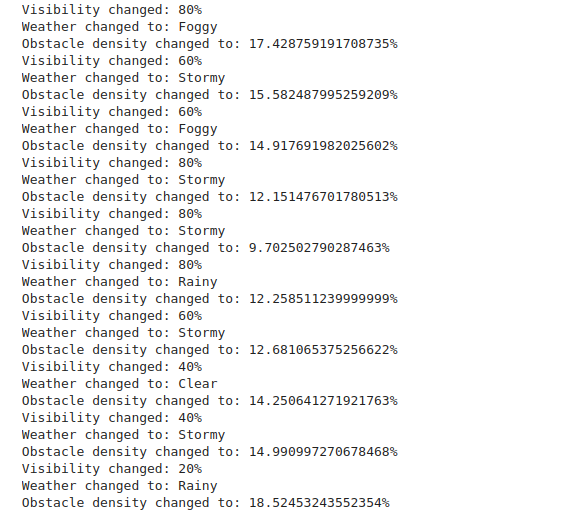
\includegraphics[width=0.7\textwidth]{2_a.png} 
    \caption{Screenshot of the output}
\end{figure}
\subsection{Adapting to Unpredictable Conditions in Maritime Navigation}

The ocean is inherently unpredictable, with various challenges such as rogue waves, unpredictable weather patterns, marine life, and shifting ocean currents. An AI system for maritime navigation must be designed to adapt to these ever-changing conditions to maintain safety and efficiency. Here's how the AI can adapt:

\subsubsection{\large Handling Rogue Waves}
Rogue waves are sudden, massive waves that can appear without warning. To adapt, the AI system could:
\begin{itemize}
    \item Continuously monitor ocean conditions using radar, sonar, and weather data.
    \item Adjust ship speed and course based on real-time data to avoid being caught in such waves.
    \item Increase the stability of the ship by adjusting the ship's trim and ballast control to handle rough seas.
\end{itemize}

\subsubsection{\large Navigating in Unpredictable Weather}
The weather in the open ocean can change rapidly, especially with storms or fog, which can severely reduce visibility. The AI should:
\begin{itemize}
    \item Continuously receive weather forecasts and live weather data (e.g., temperature, wind speed, and humidity).
    \item Adjust speed and course depending on the severity of the weather, increasing caution during storms and reducing speed during foggy conditions to avoid collisions.
    \item Monitor air pressure and temperature fluctuations to predict sudden weather changes like thunderstorms.
\end{itemize}

\subsubsection{\large Marine Life and Underwater Obstacles}
Underwater obstacles, such as rocks or submerged marine life, can pose significant threats to navigation. The AI should:
\begin{itemize}
    \item Use sonar to scan underwater surroundings for potential hazards and adjust the ship’s course to avoid them.
    \item Learn from historical data (e.g., areas where marine life is more likely to be present) to predict potential encounters with marine animals.
\end{itemize}

\subsubsection{\large Real-time Decision-making}
The AI system should continuously adjust its decision-making process based on real-time data, ensuring the ship can handle sudden changes in environmental conditions. This can be done by:
\begin{itemize}
    \item Combining input from multiple sensors (radar, sonar, GPS, weather data) to make decisions.
    \item Implementing a multi-layered decision framework that prioritizes safety (e.g., avoiding collisions) over efficiency (e.g., optimizing speed).
    \item Introducing predictive algorithms that use past environmental data to forecast potential risks, allowing for proactive adjustments.
\end{itemize}

\subsubsection{\large Long-Term Adaptation}
The system should also be able to adapt to longer-term environmental patterns, such as changes in ocean currents or regular storm paths. This could include:
\begin{itemize}
    \item Utilizing machine learning algorithms to detect patterns in historical environmental data (e.g., weather and sea conditions) and predict future changes.
    \item Dynamically adjusting the navigation route based on patterns in weather or ocean currents to avoid regions known for unpredictable conditions.
\end{itemize}

\subsubsection{\large Efficiency and Fuel Management}
As the ship adapts to unpredictable conditions, the AI should also aim to balance safety with fuel efficiency:
\begin{itemize}
    \item The AI can adjust the speed based on fuel consumption algorithms, ensuring that safety measures (like slowing down) do not overly impact the overall journey time or fuel efficiency.
    \item Route optimization should consider not just safety but also fuel consumption, avoiding detours that could lead to excess fuel use while still ensuring the ship remains safe.
\end{itemize}

By constantly evaluating and adapting to the changing ocean environment, the AI system can ensure the safe and efficient navigation of autonomous ships.

\subsubsection{\large Python Code for Adaptive Navigation System}

Here’s the Python function simulating an adaptive algorithm for the ship’s navigation system. This function adjusts the ship’s course based on real-time data about obstacles and environmental conditions.

\begin{verbatim}
import random
import math

class AdaptiveNavigationSystem:
    def __init__(self, initial_course=0, visibility=100, weather='Clear', obstacle_density=0.1):
        self.course = initial_course  # Ship's current course (angle in degrees)
        self.visibility = visibility  
        self.weather = weather 
        self.obstacle_density = obstacle_density  # Fraction of obstacles in the area (0 to 1)
        self.max_course_change = 15  # Max allowed course change in degrees for safety

    def update_conditions(self, visibility, weather, obstacle_density):
        # Update environmental conditions.
        self.visibility = visibility
        self.weather = weather
        self.obstacle_density = obstacle_density

    def assess_obstacles(self):
        # Simulate detection of obstacles and adjust course accordingly.
        if self.obstacle_density > 0.5:  
            print("High obstacle density detected. Adjusting course to avoid collisions.")
            return random.randint(-self.max_course_change, self.max_course_change)
        return 0  

    def assess_weather(self):
        # Simulate weather-based course adjustment.
        if self.weather == 'Stormy': 
            print("Storm detected. Altering course to avoid storm.")
            return random.randint(-self.max_course_change, self.max_course_change)
        elif self.weather == 'Foggy' and self.visibility < 40:
            print("Low visibility due to fog. Adjusting course for safety.")
            return random.randint(-self.max_course_change // 2, self.max_course_change // 2)
        return 0  

    def navigate(self):
        # Adjust the ship's course based on real-time data.
        course_adjustment = self.assess_obstacles() + self.assess_weather()

        if course_adjustment != 0:
            self.course += course_adjustment
            self.course = max(0, min(360, self.course))  # Ensure the course stays within 0-360 degrees
            print(f"New course: {self.course}°")
        else:
            print(f"Course remains the same: {self.course}°")
        
    def simulate_navigation(self, iterations=5):
        # Simulate a series of course adjustments over time.
        for i in range(iterations):
            print(f"\nIteration {i+1}:")
            # Simulate random updates to environmental conditions
            new_visibility = random.randint(20, 100)
            new_weather = random.choice(['Clear', 'Foggy', 'Stormy'])
            new_obstacle_density = random.uniform(0, 1)
            
            # Update conditions
            self.update_conditions(new_visibility, new_weather, new_obstacle_density)
            print(f"Updated conditions: Visibility={self.visibility}%, 
            Weather={self.weather}, Obstacle Density={self.obstacle_density * 100}%")
            self.navigate()

nav_system = AdaptiveNavigationSystem(initial_course=90, visibility=80,
weather='Clear', obstacle_density=0.2)
nav_system.simulate_navigation(iterations=5)
\end{verbatim}

This code simulates the adaptive navigation system, adjusting the ship's course based on real-time environmental data and obstacles.
\subsubsection{Output}
Here is the screenshot of the program's output:
\\ \\ \\ \\ \\ \\ \\ \\ \\ \\ \\ \\ \\ \\ \\ \\ \\ \\ \\
\begin{figure}[h!]
    \centering
    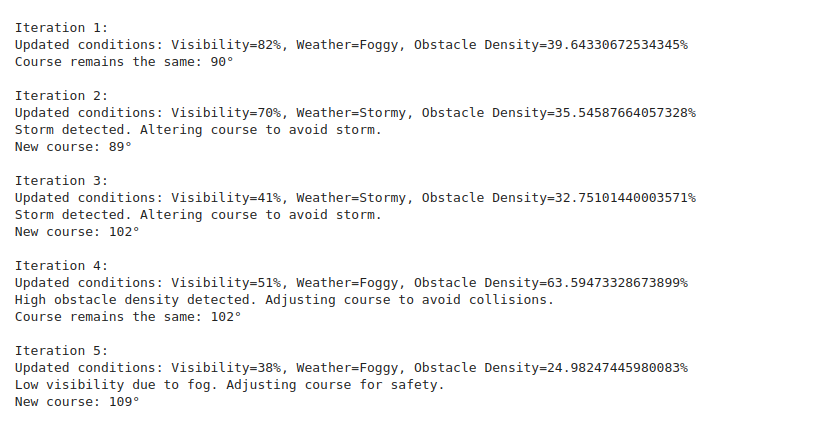
\includegraphics[width=0.7\textwidth]{2_b.png} 
    \caption{Screenshot of the output}
\end{figure}
\subsection{\large Decision-Making Without Standardized Lane Markings in Maritime Navigation}

In maritime environments, the absence of standardized lane markings, similar to those on roads for vehicles, creates unique challenges for AI-driven ships. Ships must navigate vast open waters, often in congested or poorly marked areas, such as busy ports, narrow channels, or areas with high maritime traffic. Here's how the lack of standard lane markings affects decision-making and what strategies can be implemented for safe navigation:

\subsubsection{\large Challenges Without Standardized Lane Markings}
\begin{itemize}
    \item \textbf{Uncertainty in Path Guidance}: Without defined lanes, AI systems cannot rely on visual markers or pre-determined paths to guide navigation. This means that ships must make real-time decisions based on surrounding conditions, such as traffic, obstacles, and weather. The AI must dynamically adjust its course based on these variables.
    \item \textbf{Increased Risk of Collisions}: The absence of standardized lanes increases the complexity of managing safe distances between vessels. Ships must use other data sources, like radar and AIS (Automatic Identification Systems), to detect and avoid potential collisions. However, in congested or poorly marked areas, these systems alone might not be enough, requiring more advanced decision-making algorithms.
    \item \textbf{Environmental Adaptability}: Navigating without lane markings means that the AI must also account for constantly changing environmental conditions, such as tides, currents, and weather. The absence of standard lanes makes these factors even more influential in determining the safest route, particularly in dense maritime traffic.
\end{itemize}

\subsubsection{\large Strategies for Safe Navigation in Congested Routes}
\begin{itemize}
    \item \textbf{Traffic Density-Based Decisions}: The AI system must assess the level of traffic in its vicinity and adapt its speed and course accordingly. For instance:
    \begin{itemize}
        \item \textbf{High Traffic Density}: The AI can reduce speed and alter course to avoid congested areas or navigate around other ships.
        \item \textbf{Low Traffic Density}: The AI can maintain its course and speed for more efficient navigation.
        \item \textbf{Moderate Traffic Density}: The AI should stay alert and maintain a balance between speed and course adjustments to avoid any sudden risks.
    \end{itemize}
    \item \textbf{Weather and Environmental Adaptation}: The AI must continuously monitor weather conditions and adjust navigation parameters:
    \begin{itemize}
        \item \textbf{In Stormy or High-Wind Conditions}: The AI could slow down and choose a detour to navigate through calmer waters.
        \item \textbf{In Foggy Weather}: The AI may increase sensor sensitivity (e.g., radar, sonar) to detect nearby vessels and obstacles, while proceeding with caution.
        \item \textbf{In Clear Weather}: The AI can operate at optimal speed and maintain a direct course towards the destination.
    \end{itemize}
    \item \textbf{Obstacle Detection and Avoidance}: If obstacles are detected, the AI should make immediate course corrections to avoid collisions. This can be achieved by using radar, sonar, and other sensors. In the case of large obstacles, the AI might decide to take a detour, while smaller obstacles might only require minor adjustments.
    \item \textbf{Adaptive Course Adjustments}: The AI should always be ready to adjust its course based on the real-time data collected from environmental sensors. If the ship encounters an obstacle or a change in weather, the AI can decide to slow down, take a detour, or alter its speed and direction to maintain safe navigation.
    \item \textbf{Dynamic Route Planning}: In the absence of fixed lanes, the AI should constantly evaluate its route using algorithms that consider the ship’s current position, the destination, environmental conditions, and traffic density. These dynamic adjustments help maintain a safe and efficient course.
\end{itemize}

\subsubsection{Example Decision-Making Algorithm}

The provided code simulates a decision-making process that accounts for various factors like weather, traffic density, and obstacles. Here's how the algorithm works:

\begin{itemize}
    \item \textbf{Obstacle Handling}: If obstacles are detected, the AI will take actions like maneuvering to avoid them.
    \item \textbf{Weather-Based Decisions}:
    \begin{itemize}
        \item In stormy or high-wind conditions, the AI slows down and looks for safer paths.
        \item In foggy conditions, the AI increases sensor sensitivity and proceeds cautiously.
        \item In clear weather, the AI operates at normal speed.
    \end{itemize}
    \item \textbf{Traffic-Based Decisions}:
    \begin{itemize}
        \item In high-traffic areas, the AI slows down and avoids congested routes.
        \item In moderate traffic, the AI maintains speed but stays alert.
        \item In low traffic, the AI keeps its course and speed.
    \end{itemize}
    \item \textbf{Scenario Reactions}:
    \begin{itemize}
        \item Scenario 1: In clear weather and low traffic, the ship can maintain its speed and direct course.
        \item Scenario 2: In stormy weather, high traffic, and large obstacles, the AI takes evasive actions, slows down, and alters its route to avoid collision and safer navigation.
        \item Scenario 3: In foggy weather with moderate traffic and small obstacles, the AI increases sensor sensitivity, proceeds cautiously, and adjusts course to avoid obstacles.
    \end{itemize}
\end{itemize}

\subsubsection{Code Implementation}

Here is the implementation of the decision-making algorithm in Python:

\begin{verbatim}
WEATHER_CONDITIONS = ["clear", "fog", "storm", "high-wind"]
TRAFFIC_DENSITY = ["low", "moderate", "high"]
OBSTACLES = ["none", "small", "large"]  

class AutonomousShip:
    def __init__(self, current_position, destination, speed, weather, traffic_density, obstacles):
        self.current_position = current_position
        self.destination = destination
        self.speed = speed
        self.weather = weather
        self.traffic_density = traffic_density
        self.obstacles = obstacles
        self.route = []

    def decide_route(self):
        #Decides the safest route based on traffic, weather, obstacles, and current position.
        # If there are obstacles, first take action to avoid them
        if self.obstacles != "none":
            self.route.append("maneuver to avoid obstacles")

        # Weather-based decision-making
        if self.weather == "storm" or self.weather == "high-wind":
            self.route.append("slow down")
            self.route.append("take detour to safer waters")
        elif self.weather == "fog":
            self.route.append("increase sensor sensitivity")
            self.route.append("proceed with caution")
        elif self.weather == "clear":
            self.route.append("maintain speed and course")

        # Traffic-based decision-making
        if self.traffic_density == "high":
            self.route.append("reduce speed")
            self.route.append("adjust course to avoid congestion")
        elif self.traffic_density == "moderate":
            self.route.append("maintain speed but stay alert")
        elif self.traffic_density == "low":
            self.route.append("maintain speed")

        # Final action to proceed towards the destination
        self.route.append(f"navigate towards {self.destination}")

    def display_route(self):
        print(f"Ship at {self.current_position} heading to {self.destination}")
        print("Recommended Actions:")
        for action in self.route:
            print(action)
# Scenario 1: Ship in clear weather and low traffic with no obstacles
ship1 = AutonomousShip(current_position="Port A",
destination="Port B", speed=20, weather="clear", traffic_density="low", obstacles="none")
ship1.decide_route()
ship1.display_route()

# Scenario 2: Ship in stormy weather with high traffic and large obstacles
ship2 = AutonomousShip(current_position="Port C", 
destination="Port D", speed=15, weather="storm", traffic_density="high", obstacles="large")
ship2.decide_route()
ship2.display_route()

# Scenario 3: Ship in foggy weather with moderate traffic and small obstacles
ship3 = AutonomousShip(current_position="Port E",
destination="Port F", speed=18, weather="fog", traffic_density="moderate", obstacles="small")
ship3.decide_route()
ship3.display_route()
\end{verbatim}

\subsubsection{Output}
Here is the screenshot of the program's output:
\begin{figure}[h!]
    \centering
    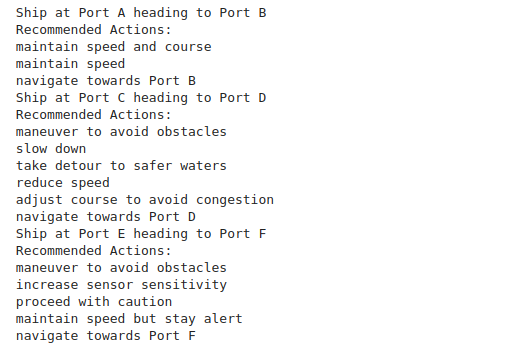
\includegraphics[width=0.7\textwidth]{2_c.png} 
    \caption{Screenshot of the output}
\end{figure}

\end{document}
